\documentclass[11pt,a4paper]{article}
\usepackage{float}
\usepackage{verbatim}
\usepackage{subfig}
\usepackage[T1]{fontenc}
\usepackage[utf8]{inputenc}
\usepackage{geometry}
\usepackage{enumitem}
%\geometry{verbose,lmargin=2cm,rmargin=2cm, bmargin=2cm, tmargin=2cm}
\usepackage{wrapfig}
\usepackage{tikz}
\usetikzlibrary{decorations.markings}
\usepackage{calc}
\usepackage{wrapfig}
\usepackage{graphicx}
\usepackage{amssymb}
\usepackage{amsmath}
\usepackage{esint}
\usepackage{multicol}
\usepackage{hyperref}
\usepackage{listings}
\hypersetup{
    colorlinks=true,
    linkcolor=blue,
    filecolor=magenta,
    urlcolor=cyan,
}
\usepackage{listings}
\lstset{ %
  backgroundcolor=\color{white},   % choose the background color; you must add \usepackage{color} or \usepackage{xcolor}; should come as last argument
  basicstyle=\footnotesize,        % the size of the fonts that are used for the code
  breakatwhitespace=false,         % sets if automatic breaks should only happen at whitespace
  breaklines=true,                 % sets automatic line breaking
  captionpos=t,                    % sets the caption-position to bottom
  commentstyle=\color{teal},    % comment style
  deletekeywords={...},            % if you want to delete keywords from the given language
  escapeinside={\%*}{*)},          % if you want to add LaTeX within your code
  extendedchars=true,              % lets you use non-ASCII characters; for 8-bits encodings only, does not work with UTF-8
  frame=single,                    % adds a frame around the code
  keepspaces=true,                 % keeps spaces in text, useful for keeping indentation of code (possibly needs columns=flexible)
  keywordstyle=\color{blue},       % keyword style
 % language=Python,                 % the language of the code
  morekeywords={*,...},           % if you want to add more keywords to the set
  numbers=left,                    % where to put the line-numbers; possible values are (none, left, right)
  numbersep=5pt,                   % how far the line-numbers are from the code
  numberstyle=\tiny\color{black}, % the style that is used for the line-numbers
  rulecolor=\color{black},         % if not set, the frame-color may be changed on line-breaks within not-black text (e.g. comments (green here))
  showspaces=false,                % show spaces everywhere adding particular underscores; it overrides 'showstringspaces'
  showstringspaces=false,          % underline spaces within strings only
  showtabs=false,                  % show tabs within strings adding particular underscores
  stepnumber=1,                    % the step between two line-numbers. If it's 1, each line will be numbered
  tabsize=2,                       % sets default tabsize to 2 spaces
  title=\lstname                   % show the filename of files included with \lstinputlisting; also try caption instead of title
}
\begin{document}



%\preprint{APS/123-QED}

\title{FYS2150 \\ Lab Report: Drag}% Force line breaks with \\

\author{Nicholas Karlsen}
% \email{nichoka@student.matnat.uio.no}

\date{\today}% It is always \today, today,
             %  but any date may be explicitly specified

\maketitle

\begin{abstract}
  Studying the type of fluid flow of an assortment of spheres of varying mass and diameter in a fluid by the use of image processing. Then comparing the data looking for possible links between flow type and the physical parameters of the spheres.
\end{abstract}

%\tableofcontents

\section{\label{sect:intro}Introduction}
  This report contains a summary of the experiment performed in the lab 21.03.2018 concerning the flow of several spherical objects in a range of different sizes and densities and the subsequent analysis of the data afterwards. 

  The balls were immersed in an oil, dropped and filmed. Post-lab, the raw footage was then processed using a Python script in order to quantify the motion of the spheres and determine the type of flow undertaken by spheres based on their terminal velocity. 

  There was found to be a possible correlation between the the type of flow, and the size of balls with the same density. But no such correlation was found for balls of similar size, but different densities.

\section{\label{sect:theory}Theory}

  \subsection{Fluid dynamics}
    \subsubsection{Forces}
    For a body falling vertically under gravity, there are primarily three forces acting. Gravity, Upthrust and Drag. Gravity is expressed quite simply by $F_g = mg$, where $m$ denotes the mass of the body and $g$ the acceleration due to gravity, which is for the purposes of this report is taken to be equal to $9.80665$ms$^{-2}$ \cite{wiki:grav}. 

    Upthrust is given by Archimedes principle, and stated mathematically in Eqn. \ref{eqn:archi}, where $V$ denotes the volume of the body and $\rho$ the density of the medium in which the body is submerged.

    \begin{equation}
      F_u = \rho V g
      \label{eqn:archi}
    \end{equation}

    Lastly, drag, $F_d$. The drag force is quite a complex one, as its form varies depending on the type of flow which the body is undertaking, which is either idealized, laminar flow with straight, continuous field lines or turbulent flow, with chaotic field lines.
    In equilibrium, when the body is traveling at constant velocity, the relationship between the forces is given by Eqn. \ref{eqn:equil}, which means that $F_d$ can be expressed in terms of $F_g$ and $F_u$.
    
    \begin{equation}
      \sum F = F_g - F_u - F_d = 0
      \label{eqn:equil}
    \end{equation}
    Enabling us to study the drag force by making measurements of the comparatively simple forces, gravity and upthrust while the system is in a state of equilibrium.

    \subsubsection{\label{sec:fluflo}Types of flow}
    \begin{equation}
      R_e = \frac{\rho v r}{\mu}
      \label{eqn:rey}
    \end{equation}
    The Reynolds number, $R_e$ given by Eqn. \ref{eqn:rey} is a dimensionless variable used to quantify different types of flow, where $v$ denotes the velocity of the body flowing in the liquid, $r$ its radius, $\rho$ the density of the liquid and $\mu$ its viscosity. A lower Reynolds number indicated laminar flow, whilst a higher indicates turbulent flow.

    Further, two additional dimensionless variables, $C_R$ and $C_S$ can be found \cite{question_paper} through dimensional analysis, given in Eqn \ref{eqn:dimvar}
    \begin{align}
      \begin{split}
        C_R &= \frac{F_d}{\rho v^2 r^2} \\
        C_S &= \frac{F_d}{\mu v r}
      \end{split}
      \label{eqn:dimvar}
    \end{align}
    where $C_R$ correlates to $F_d$ which is independent of the viscosity of the fluid, equivalent with a high Reynolds number and meaning that the flow is more turbulent than it is laminar and is referred to as Rayleigh flow. The opposite is given by $C_S$, which correlates to $F_d$ which is dependent on the viscosity of the fluid, equivalent with a low Reynolds number. This implies that the flow is more laminar than it is turbulent, and is referred to as Stokes' flow.

    And lastly, for Stokes' flow $F_d/r \propto v$ and for Rayleigh flow $F_d / r^2 \propto v^2$. \cite{question_paper}
    


  \subsection{Image processing\label{sect:imgpro}}
      \begin{equation}
        Y_{i, j} = 0.2126\cdot\textup{I}_{i, j, 1} 
        + 0.7152\cdot\textup{I}_{i, j, 2} 
        + 0.0722\cdot\textup{I}_{i, j, 3}
        \label{eqn:rgb2gray}
      \end{equation}
      An image can be represented by an $M \times N$ array, where each entry, $\textup{I}_{i, j}$ is a list of varying length depending on the color space of the image, consisting of numbers from 0 to 256, signifying the intensity of each color. RGB 3 entries and gray scale 1 entry. Conversion from RGB to gray scale is calculated by Eqn. \ref{eqn:rgb2gray} where I$_{i, j, ...}$ denotes array elements of the input RGB image and Y$_{i, j}$ the output gray scale image. \cite{wiki:grayscale}
      \newline
      A gray scale image can be further simplified by converting it to a binary black or white image. i.e, an image consisting only of black or white pixels. Such an image can be created by Eqn. \ref{gray2bin} where $X_{i, j}$ denotes the array element of the output binary image and T the threshold, a number between 1 and 256.
      \begin{equation}
        X_{i, j} = \left\{ 
        \begin{matrix}
          Y_{i,j} \geq T & 256 \\
          Y_{i, j} < T & 0
        \end{matrix}
        \right.
        \label{gray2bin}
      \end{equation}
      The properties of a binary image can then be determined by an algorithm such as \lstinline{regionprops()} which determines the properties of shapes present in the image. For the purposes of analyzing a video, and finding the position of one particular shape in each frame of that video, it is important that the binary image only contains one shape and minimal noise, else \lstinline{regionprops()} may not work as desired.

      In order to achieve this, two methods in particular are easy to implement. 1) If the object moves in an "open" area, cropping the image may suffice as a way to filter out anything undesirable. This is the most efficient method as far as computation time is concerned. It does however limit the possibility of completely automating the analysis of a large quantity of videos. 2) If the background is entirely static, or almost. The background can be filtered out by multiplying each frame of the video by an inverted image of the background divided by 256. Such an inverted image will have value 0 where the static objects are located, and 1 everywhere else.

      An example an image processed using the technique described in this section in shown in Fig. \ref{fig:vid_frame}

      \begin{figure}[H]
        \center
        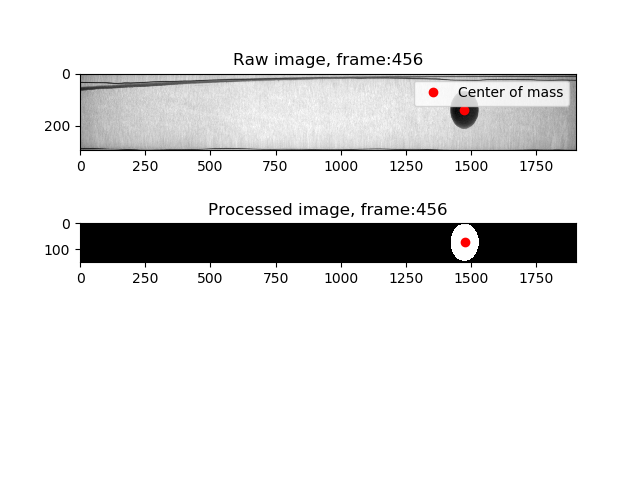
\includegraphics[scale=0.75]{scripts/figs/graphs/B1_1.png}
        \caption{Unprocessed and processed frame from one of the recordings.}
        \label{fig:vid_frame}
      \end{figure}


\section{\label{section:experimental}Experimental Procedure} 
  
  \subsection{Video capture\label{subsect:vidcap}}
    
    \begin{figure}[H]
      \center
      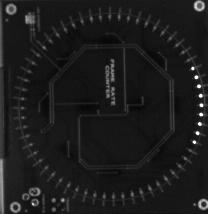
\includegraphics[width=7cm]{scripts/figs/sync_fps.png}
      \caption{Signal used to determine the FPS of the camera}
      \label{fig:FpsSignal}
    \end{figure}
  
    In order to capture the motion of the balls, a USB video camera was connected to a computer running uEye cockpit\cite{_ueye_????}, a program which allowed us to change the settings of the camera, as well as record video files. The image was set to gray-scale and the contrast, exposure, gain etc was changed such that the color histogram in uEye would show two significant, separated peaks such that it would be easy to process the image using the method described in section \ref{sect:imgpro}.

    Next, the error of the set FPS of the camera had to be determined. This was done by connecting a series of LEDs in a circle (see Fig. \ref{fig:FpsSignal}) to a signal generator. The light emitted would "circle" at a rate which could be changed using the signal generator. By adjusting the rate such that the emitted light would seem stationary when observed through the video feed in uEye, the true FPS of the camera could be determined. In our test, we set the camera to film at 60 FPS and the rate was adjusted untill the period of the LED was synced up with the camera at $3.60047$ KHz, the equivalent of $60.00783$ periods per second.

    In order to get the conversion factor between pixels and meters, a still picture was taken of the tubes with a known length in frame, at a distance roughly equal to where the balls would travel. This had to be done for each experimental setup. For our known lengths, we used a meter rule and a $30$ cm ruler for the large and small scale experiments respectively. See Fig. \ref{fig:scale1}.

    \begin{figure}[H]
      \center
      \subfloat[][Large tube]{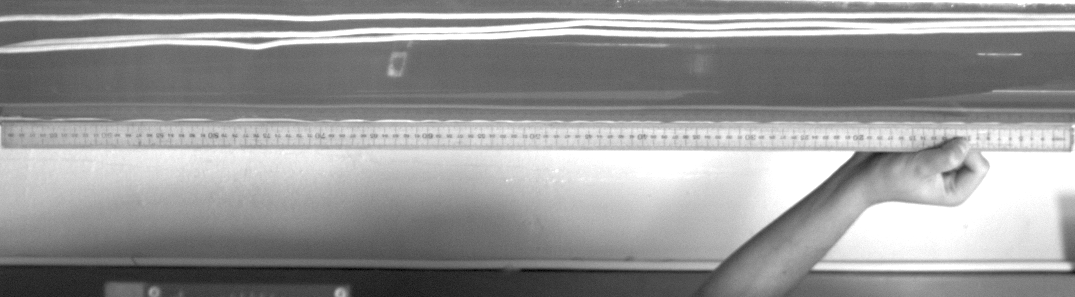
\includegraphics[width=8cm, angle=90]{scripts/figs/bilde_scale1.png}\label{<figure1>}}
      \subfloat[][Small tube]{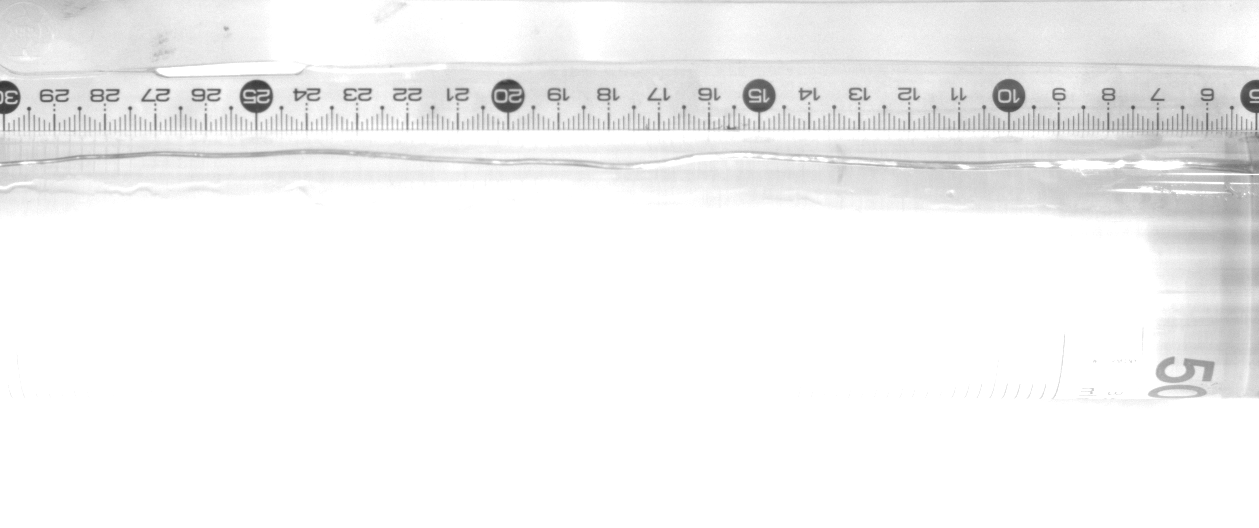
\includegraphics[width=8cm, angle=90]{scripts/figs/bilde_scale2.png}\label{<figure1>}}
      \caption{Cropped images used to find pixel to meter ratio for both of the tubes. (Scaled down in this document)}
      \label{fig:scale1}
    \end{figure}
  
  \subsection{Equipment}

    We had two similar experimental setups. One large scale, and one small scale. the large scale consisted of a roughly 2.5-3m tall\footnote{We did not measure the height of the tube, but it was fairly close to the ceiling.} transparrent tube, and the small scale a 30-40cm transparent measuring tube. Both of the tubes were filled with oil (Shell Tellus S2 M 68 Industrial Hydraulic Fluid\cite{_shell_????}).

    The set of balls which were to be dropped in the large scale setup are depicted in Fig. \ref{fig:balls}. Additionally, there were two smaller balls which were dropped in the small scale setup. The mass of the balls was measured using a digital scale with a precision of $0.01$g \cite{_proscale_????}, except for the two smallest balls, for which the mass was given by the lab instructor. The diameter of the balls was measured using a Vernier Caliper with a precision of $0.01$mm, again, except for the two smallest balls, which diameter was provided by the lab instructor.

    \begin{figure}[H]
      \center
      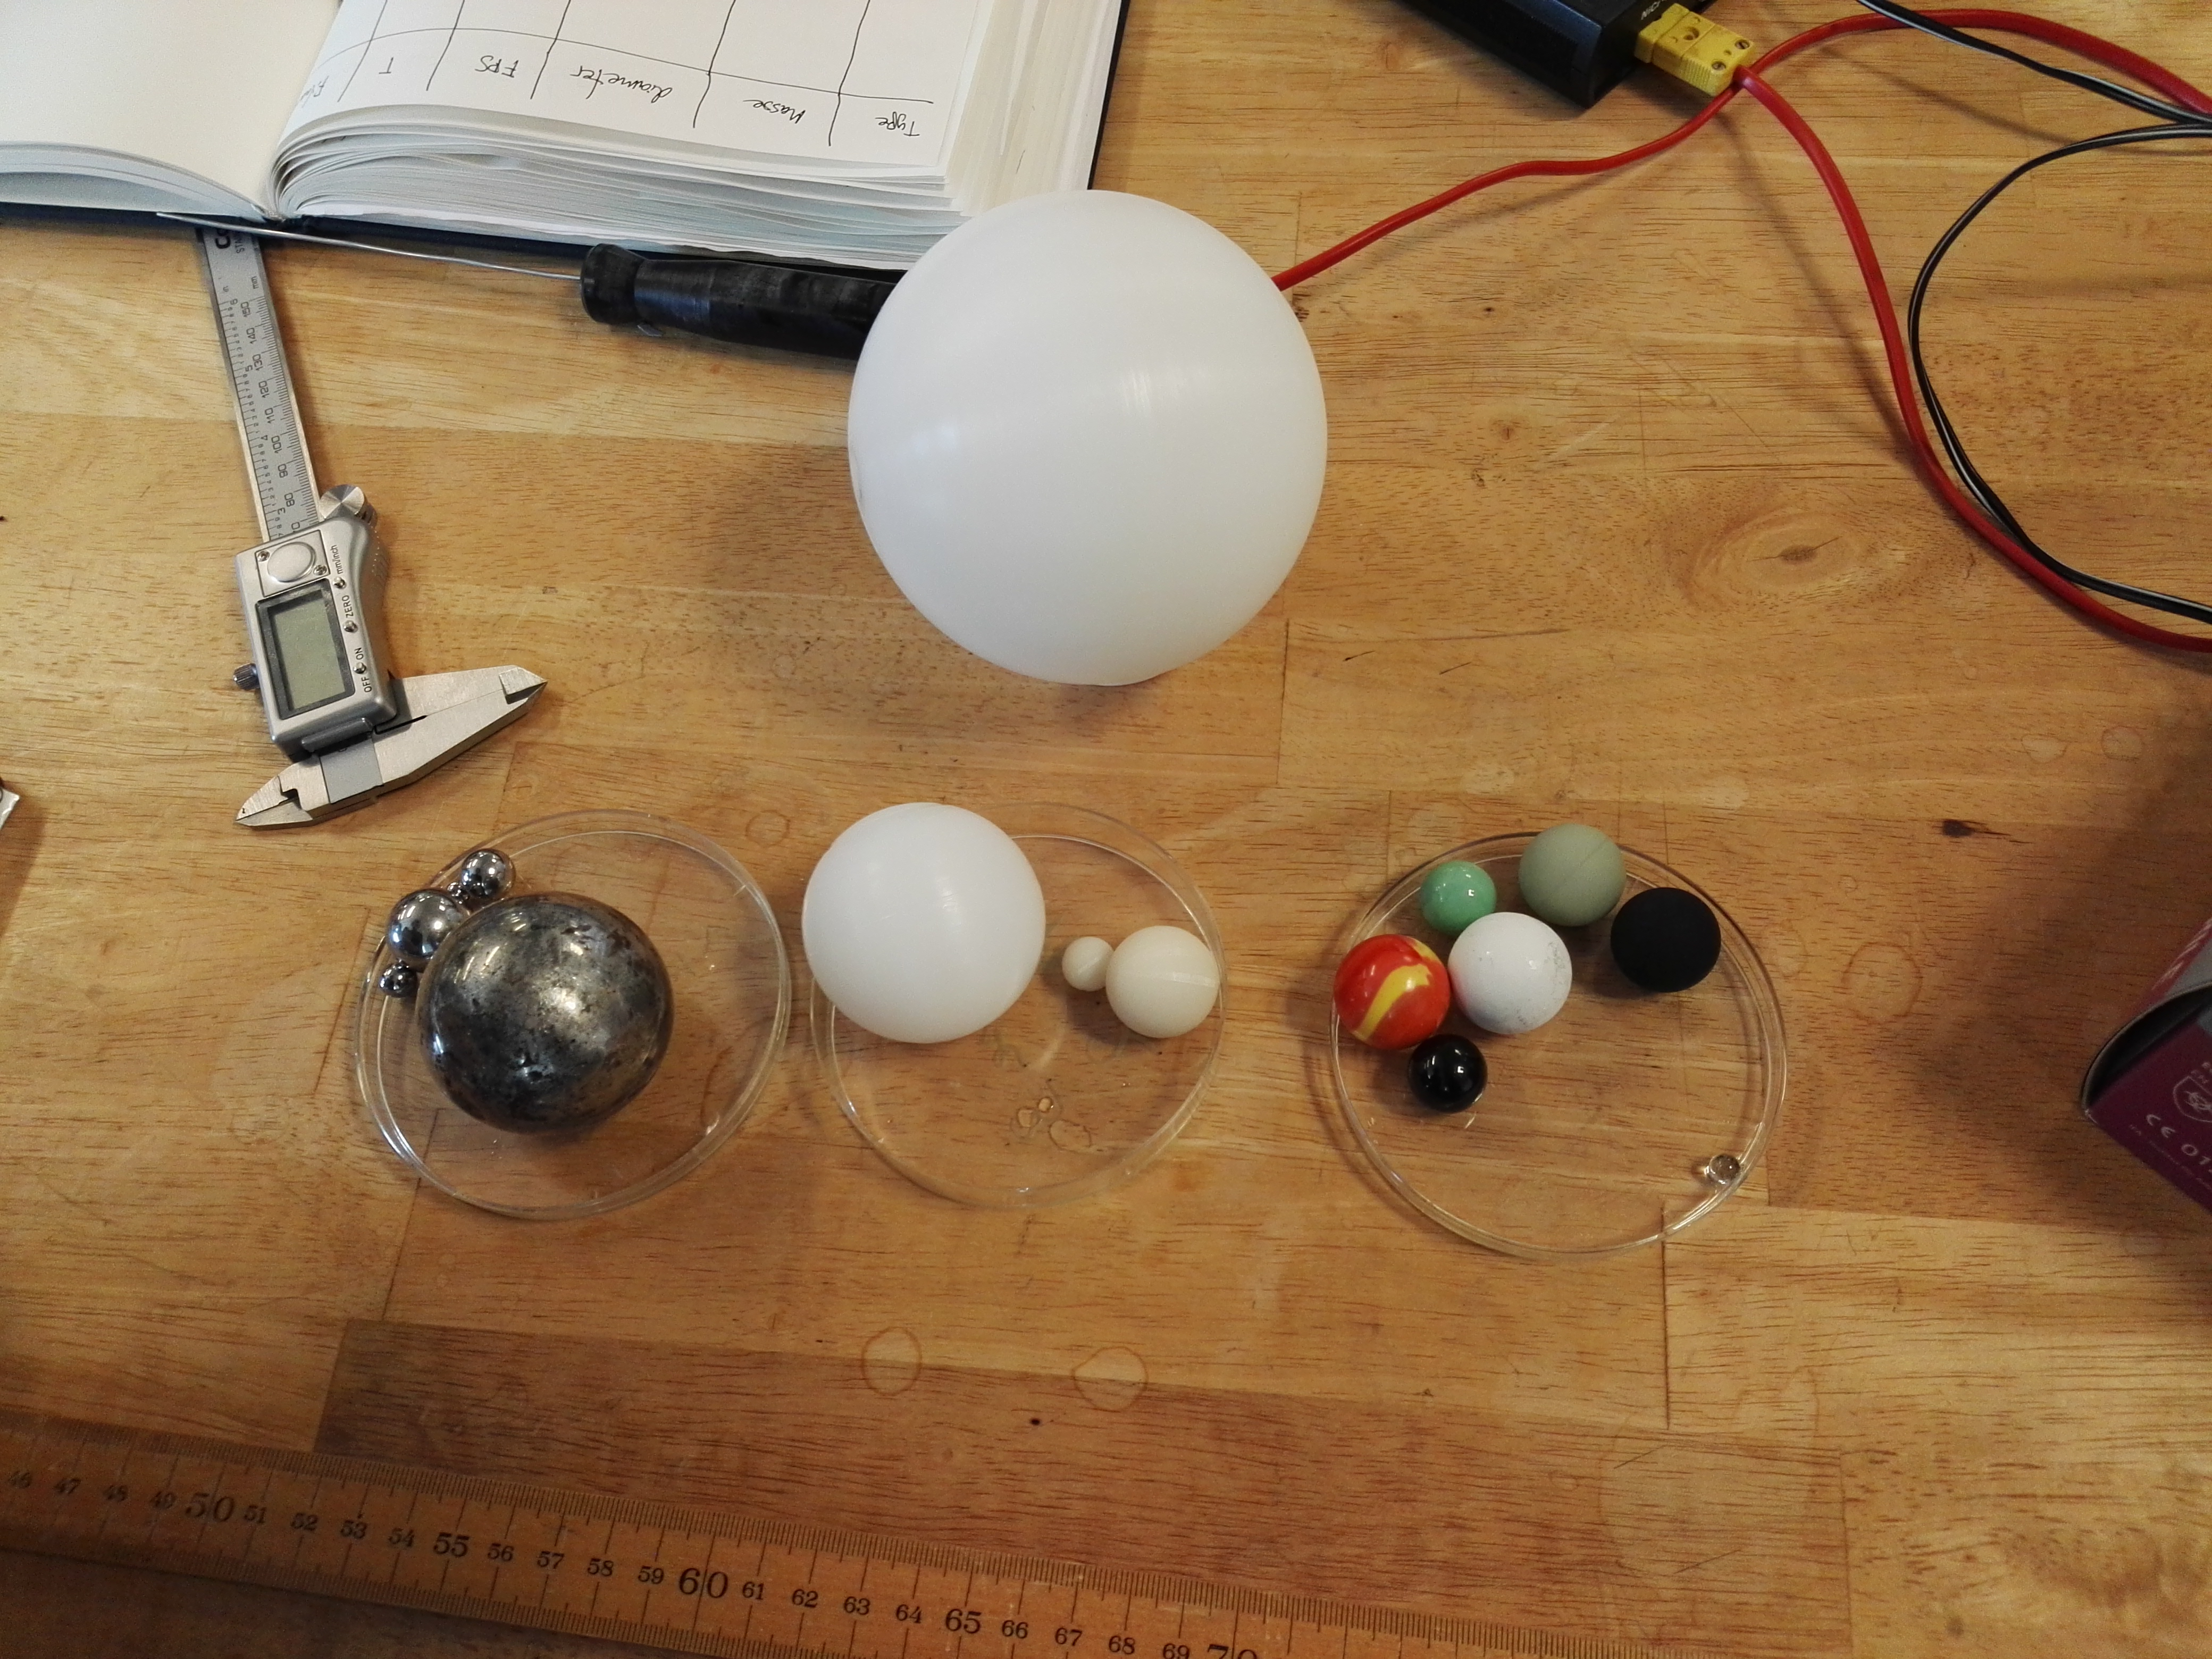
\includegraphics[width=7cm]{scripts/figs/IMG_20180321_131204.jpg}
      \caption{Most of the balls used in the experiment, excluding the ones labeled small 1 and 2.}
      \label{fig:balls}
    \end{figure}

  \subsection{Procedure}
    The experiment was performed by 3 people performing 3 different, simultaneous tasks. It can technically be performed by one person, but due to the nature of the experiment, it is not recommended, as it is not practical to make repeated readings if something goes wrong.

    The camera was pointed towards the large-scale tube, and prepared as described in section \ref{subsect:vidcap} between each reading. It was important that the lighting in the room was fairly constant for the video capture, so curtains were put in front of the windows. The camera was kept at 100 FPS for every experiment. For some of the balls with relatively low terminal velocity, the FPS could have been lowered to save space without making any significant sacrifices to the accuracy, but as we did not have any predicted values for the terminal velocity of the individual balls, we opted to keep it at 100FPS for every single experiment.

    Before each experiment, the temperature of the oil was measured using an IR-thermometer with an accuracy of $\pm2^\circ$C \cite{_fluke_????}. Which is used to determine the viscosity of the oil.

    For each experiment, a ball was picked up by hand and brought to the top of the tube by ladder. The ball was gripped tightly before carefully submerging it in the oil. After having ensured the person operating the camera software was ready to record, the ball was dropped. It was critical that the ball was dropped in a certain way, otherwise it gained too much horizontal velocity, which at worst could cause it to hit the side of the tube halfway through\footnote{Which happened in our first attempt} the tube. In order to avoid this, it is important to separate the fingers gripping the ball at the same time when dropping it, instead of letting it slide out of the hand. Sliding it out, leads it to spin, which in turn may lead it to move horizontally.

    The same procedure was performed for the small-scale experiments.


\section{\label{sect:results}Results}

  The recorded data, and some of the derived results of the experiment is given in Table \ref{tab:results} and presented graphically in Figures \ref{fig:plots1}, \ref{fig:plots2}.

  For ball "A1", the terminal velocity could not be determined as the ball was dropped poorly and hit the side of the tank. As for A6 and D2, the balls could not be distinguished from the background when performing the video analysis.
  \begin{table}[H]
    \center
    \caption{Results}
    \begin{tabular}{ r | l  l  l  l  l  l  l l  l }
      \input{scripts/data/FINAL_table.dat}
    \end{tabular}
    \label{tab:results}
  \end{table}

  \begin{figure}[H]
    \center
    \subfloat[][$v_c$ against $F_g/r$]{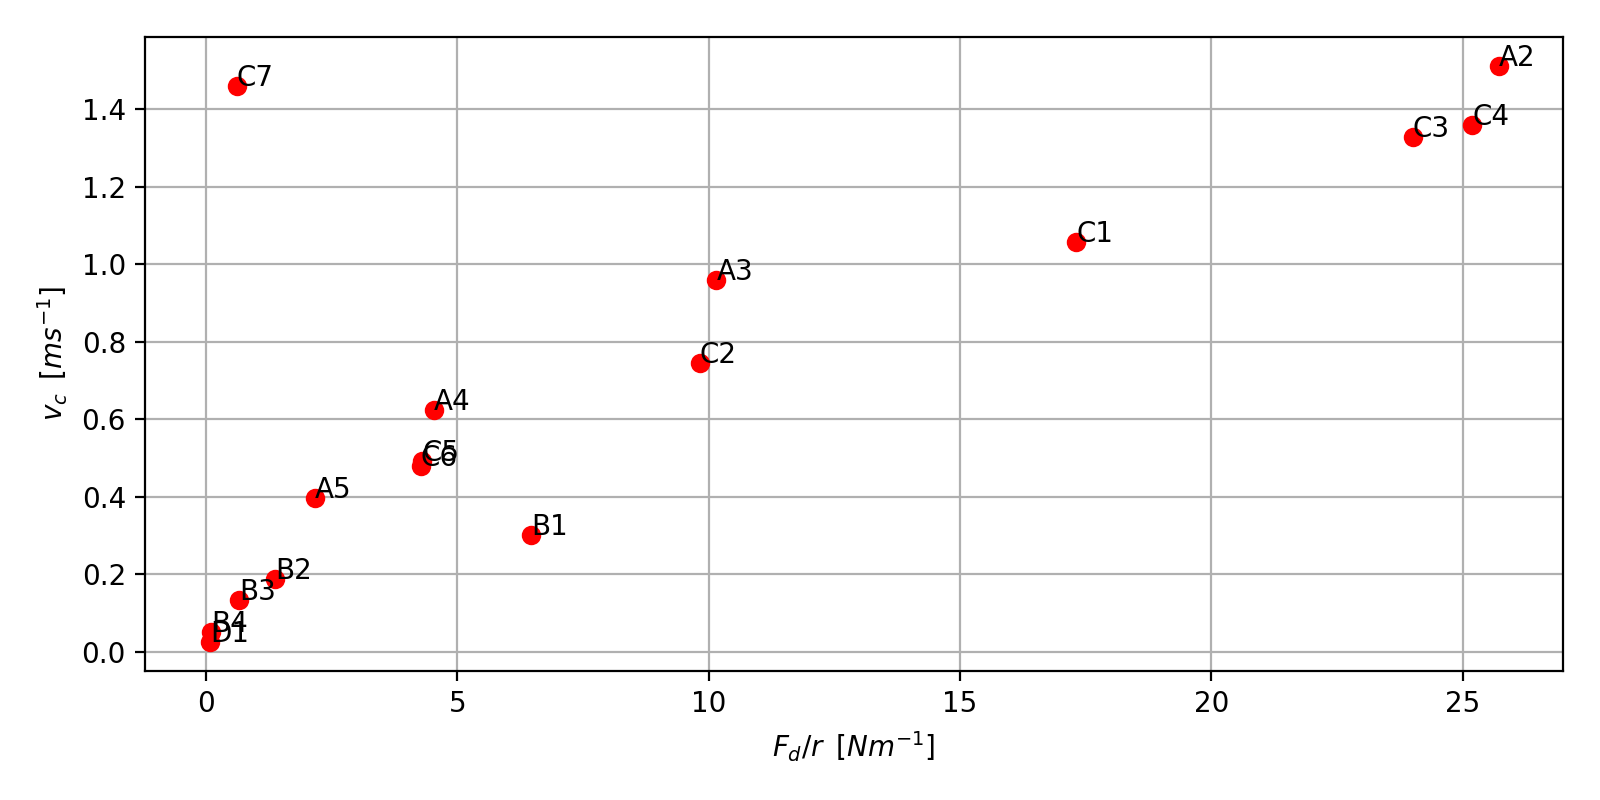
\includegraphics[scale=0.75]{scripts/figs/v_fgr.png}\label{fig:lam}}\\
    \subfloat[][$v_c^2$ against $F_g/r^2$]{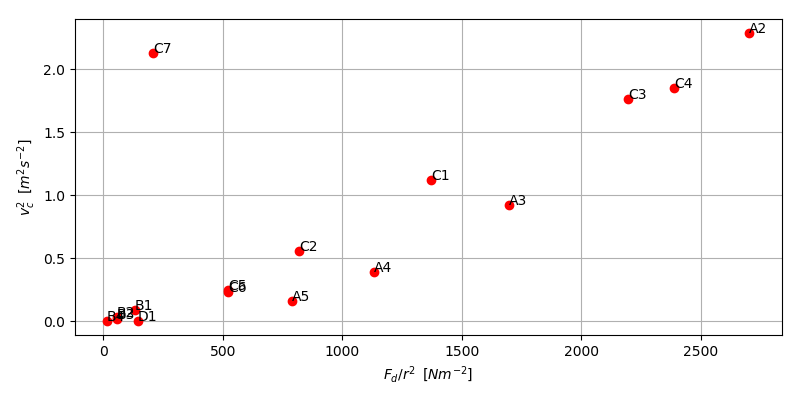
\includegraphics[scale=0.75]{scripts/figs/v2_fgr2.png}\label{fig:turb}}
    \caption{Relationship between velocty, radius and , where the annotations denote which ball the point represents}
    \label{fig:plots1}
  \end{figure}

    \begin{figure}[H]
    \center
    \subfloat[][$C_R$ against $R_e$]{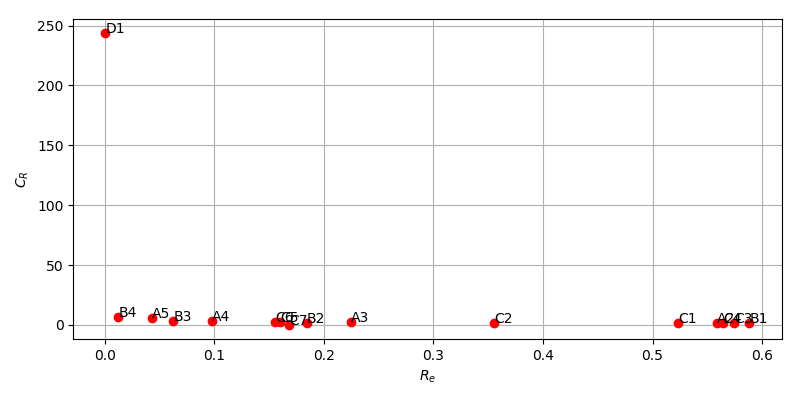
\includegraphics[scale=0.75]{scripts/figs/CR_RE.png}\label{fig:CR_RE}}
    \\
    \subfloat[][$C_S$ against $R_e$]{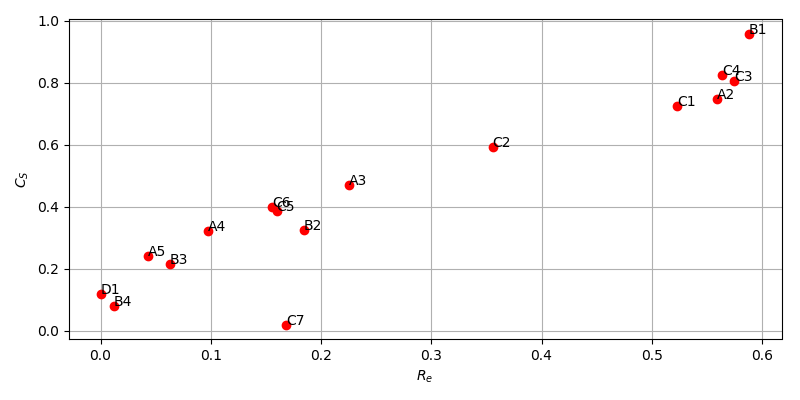
\includegraphics[scale=0.75]{scripts/figs/CS_RE.png}\label{fig:CS_RE}}
    \caption{Relationship between the dimensionless variables, $C_R$(\ref{fig:CR_RE}), $C_S$(\ref{fig:CS_RE}) and Reynolds number, where the annotations denote which ball the point represents. Note that. (Note: D1 omitted from fig \ref{fig:CR_RE} due to its relatively high value for $C_R$, see table \ref{tab:results})}
    \label{fig:plots2}
  \end{figure}




\section{\label{sect:discuss}Discussion}
  \subsection{Precision of the terminal velocity}

    When looking at the velocity/time plots for the balls, one would expect a gradually rising plot that flattens off ($\pm$ some noise) as(/if) the ball reaches its terminal velocity. However, when analyzing the data, i found that for many of the balls, the ball would reach a maximum and the subsequently begin to decelerate. This goes against what is expected, and affects the precision of the determined terminal velocity. As it turns out, this unexpected result is likely due to local changes in temperature, and therefore viscosity in the oil. Due to this disparity, the terminal velocity will also change. One could argue that recording the velocity at the same point at which the temperature was recorded would be an elegant work around to this problem, however, no such record was taken, so this point can not be determined.

    Due to this, I opted to use the largest "flat" area in the velocity time graph as my basis for finding the terminal velocity of the ball, as depicted for one of the balls in Fig. \ref{fig:D1speed}
    \begin{figure}[H]
      \center
      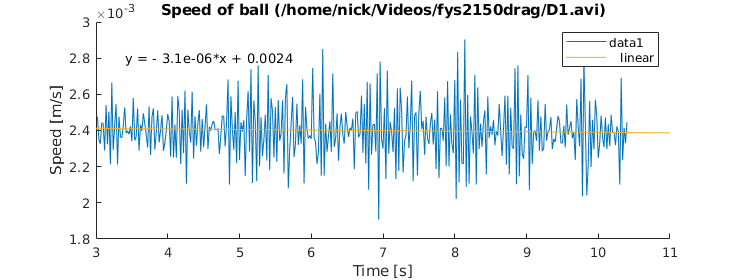
\includegraphics[scale=0.7]{scripts/figs/D1_speed.png}
      \caption{Velocity-time graph for D1, with a linear fit to determine if the acceleration is $\approx 0$}
      \label{fig:D1speed}
    \end{figure}

    In addition to the problems with the image analysis, the video also lacks some precision. The balls travel in a tube filled with oil, therefore, the light emitted from the balls will be refracted as it travels to the lens. As such, the footage captured by the camera is not an entirely precise measurement of the motion of the ball. However, the effect of refraction is likely minor compared to what was discussed above. 
    
  \subsection{Analysis}
    Due to a last minute discovery of a bug in my code, which analyzed the video files. All of my data had to be scrapped and re-analyzed using a different script\footnote{lesTolkVideo.m} during the last minute. Due to this, I did not have the time to calculate the errors for each result.

    Due to the lack of error-bars in the Fig \ref{fig:plots1}, it is difficult to place a line, showing which results are proportional to each other and which agent, as the only clear out-lier is C7, which incidentally is an out-lier in both Fig. \ref{fig:lam} and \ref{fig:turb}, suggesting that it is anomalous result. As such, I struggle to separate which balls undertake Rayleigh flow and which undertake Stoke flow based on this plot.

    Looking at Figures \ref{fig:plots2}, I see that laminar flow, a small $R_e$ implies a small $C_S$ and similarly, that a small $C_R$ implies a larger $R_e$, that the flow is more turbulent.
    Further balls seems to be predominantly split into two clusters, ignoring C7, for the reasons stated above. The most tightly knit cluster being the one at $0.5 < R_e < 0.6$. The balls in this cluster are A2, B1, C1, C3 and C4. In the case of A2 and B1 in particular, their common trait is that they are among the largest in their respective category, which are all made of the same material. Such a link is difficult to make in the case of C1 and C3, as that category contains mixed materials and are of similar sizes. I tried looking at the densities for this group, however, both C1 and C3 are of similar density to other balls in this group, so this does not separate them either.

    As far as group A and B are concerned, looking at Fig. \ref{fig:plots2}, the common trend seems to be that the flow goes towards being more laminar as their size decreases.

\section{\label{sect:conclusion}Conclusion}
  To conclude, there seems to be a correlation between the size of a sphere, and its Reynolds number for objects of the same material. For spheres of different materials and similar size, there is no obvious link between the density of the material and the Reynold number.


\bibliographystyle{plain}
\bibliography{references.bib}

%%%%%%%%%%%%%%%%%%%%%%%%
%%% END OF MAIN BODY %%%
%%%%%%%%%%%%%%%%%%%%%%%%

%\appendix*
%\section{Scripts}
%\lstinputlisting[language=python]{scripts/lesVideo_conv.py}
%\lstinputlisting{scripts/data/labdata.dat}

\end{document}